\documentclass[10pt]{article}

\usepackage[margin=0.82in]{geometry}
\usepackage[T1]{fontenc}
\usepackage{lmodern}
\usepackage{microtype}
\usepackage{amsmath,amssymb}
\usepackage{booktabs}
\usepackage{tabularx}
\usepackage{longtable}
\usepackage{array}
\usepackage{xcolor}
\usepackage{enumitem}
\usepackage{listings}
\usepackage{tikz}
\usetikzlibrary{arrows.meta,positioning,fit,shapes.geometric}
\usepackage{hyperref}

\hypersetup{
  colorlinks=true,
  linkcolor=blue!55!black,
  citecolor=blue!55!black,
  urlcolor=blue!55!black,
  pdftitle={AutoMech Technical Report}
}

\definecolor{AutoBlue}{HTML}{235789}
\definecolor{AutoTeal}{HTML}{2A9D8F}
\definecolor{AutoGold}{HTML}{E9C46A}
\definecolor{AutoRed}{HTML}{C94C4C}
\definecolor{AutoGray}{HTML}{F2F4F7}
\definecolor{CodeGray}{HTML}{F7F7F7}

\newcommand{\CodeRef}[1]{\texttt{\detokenize{#1}}}
\newcommand{\ResultBlank}{\rule{1.25cm}{0.35pt}}
\newcommand{\PendingResultsNotice}{%
  \begin{center}
  \fcolorbox{AutoRed}{AutoGray}{%
    \parbox{0.92\linewidth}{\small\textbf{No benchmark was executed for this report.}
    Every result cell below is intentionally blank. Blank does not mean zero, failure,
    missing data, or not applicable.}}
  \end{center}
}

\lstset{
  language=Python,
  basicstyle=\ttfamily\small,
  backgroundcolor=\color{CodeGray},
  frame=single,
  rulecolor=\color{black!20},
  showstringspaces=false,
  columns=fullflexible,
  keepspaces=true,
  keywordstyle=\color{AutoBlue}\bfseries,
  commentstyle=\color{black!55},
  stringstyle=\color{AutoTeal!70!black}
}

\tikzset{
  box/.style={draw, rounded corners, align=center, minimum height=8mm,
              minimum width=24mm, fill=AutoGray},
  process/.style={box, fill=AutoBlue!9, draw=AutoBlue},
  check/.style={diamond, draw=AutoTeal!80!black, fill=AutoTeal!10,
                align=center, aspect=2.0, inner sep=1.5pt},
  state/.style={box, fill=AutoGold!25, draw=AutoGold!70!black},
  flow/.style={-{Latex[length=2.2mm]}, thick},
  feedback/.style={-{Latex[length=2.2mm]}, thick, dashed, draw=AutoRed}
}

\title{\textbf{AutoMech Technical Report}\\[0.4em]
\large Executable Mechanical Reasoning for Scalable Single-Agent Text-to-CAD}
\author{AutoMech Team}
\date{Implementation snapshot: August 10, 2026}

\begin{document}
\maketitle

\begin{center}
\fcolorbox{AutoBlue}{AutoGray}{
\parbox{0.92\linewidth}{
\textbf{Report status.} This document describes an implementation snapshot, including
local changes present in the inspected working tree. It does not claim benchmark
performance. Numerical constants used by control logic are implementation settings,
not experimental measurements. The inference service is treated as an abstract
text-and-image generation interface; no provider-specific behavior is assumed.
}}
\end{center}

\begin{abstract}
Most text-to-CAD systems generate a parametric program from a natural-language request.
This direct formulation is effective for compact artifacts, but whole-machine generation
becomes fragile as assemblies grow. In mechanisms with twenty or more realized parts,
gear spacing, shaft fits, axial stations, support paths, motion frames, and transmission
relations form a dense network of dependencies. If those dependencies remain implicit in
a model's reasoning, a locally plausible coordinate can invalidate distant geometry, and
a broad rewrite can destroy parts that were already correct.

AutoMech extends whole-machine text-to-CAD around a simple principle: mechanical reasoning
that determines geometry should be expressed as executable Python. One agent authors one
complete parametric machine program. Root parameters and derived functions determine
placements and dimensions; a structured semantic sidecar records ports, relations, motion
joints, transmissions, and intended outputs. AutoMech executes the program in a
time-bounded child process, separates local part geometry from world pose, validates the
result using conservative connectivity and solid-intersection checks, evaluates physical
function, and returns localized evidence for revision. Per-iteration snapshots and
best-state rollback reduce divergence.

This report follows the architecture--framework--evaluation organization commonly used by
large-system technical reports, including the reporting pattern of OneRec~\cite{onerec}.
It documents the current implementation and defines a future evaluation protocol. All
benchmark result tables are intentionally blank pending controlled execution.
\end{abstract}

\tableofcontents
\newpage

% -----------------------------------------------------------------------------
\section{Introduction}
% -----------------------------------------------------------------------------

AutoMech maps a natural-language mechanical request to one complete executable CAD
program. The same agent defines every realized part and its global layout in a
\CodeRef{build123d} script assembled through \CodeRef{cadpy}'s
\CodeRef{AssemblyHelper}. The program contains a \CodeRef{build_machine()} function for
geometry and a \CodeRef{MECHANISM} dictionary for semantics. Execution, rather than source
plausibility, determines whether the response is a valid machine
\CodeRef{maker2/single_agent.py:1--11}.

The whole-machine formulation retains global context, but assembly scale changes the
problem. A large mechanism is not merely a longer list of primitives. Its part dimensions,
local origins, assembled transforms, fits, support relations, moving coordinate frames,
and transmission paths must remain mutually consistent. Source comments identify
watch-like mechanisms with more than twenty parts as a practical collision-preparation
workload \CodeRef{maker2/convex_decomp.py:357--362}; the revision loop also records cases
where pairwise fault lists exceeded what a short feedback message could represent
\CodeRef{maker2/single_agent.py:703--717}.

The central design decision is to move calculation out of transient model reasoning and
into executable program structure. Independent choices are declared once as root
parameters. Dependent quantities are functions of those roots. Geometry and semantic
metadata consume the same values. As a result, the generated file becomes an explicit,
inspectable record of mechanical reasoning rather than only a sequence of shape-building
commands.

AutoMech contributes the following system mechanisms:
\begin{enumerate}[leftmargin=*]
  \item an executable whole-machine representation with root parameters, derived
        mechanical functions, and structured mechanism semantics;
  \item a deterministic execution and normalization path that extracts local meshes,
        world poses, and simulator-facing metadata;
  \item a verification-guided refinement framework with actionable build errors,
        connectivity and intersection checks, physical evaluation, per-iteration
        snapshots, and regression rollback; and
  \item a reproducible evaluation protocol for buildability, scaling, physical function,
        and refinement behavior.
\end{enumerate}

Development observations motivate these mechanisms but do not establish their general
performance. The evaluation section therefore contains definitions and blank templates,
not inferred results.

% -----------------------------------------------------------------------------
\section{Architecture}
% -----------------------------------------------------------------------------

Figure~\ref{fig:architecture} summarizes the AutoMech architecture. A request is converted
into an executable machine program; child-process evaluation produces explicit geometry
and semantic state; normalized artifacts feed geometric and physical verification; and
structured evidence returns to the same authored program for revision.

\begin{figure}[ht]
\centering
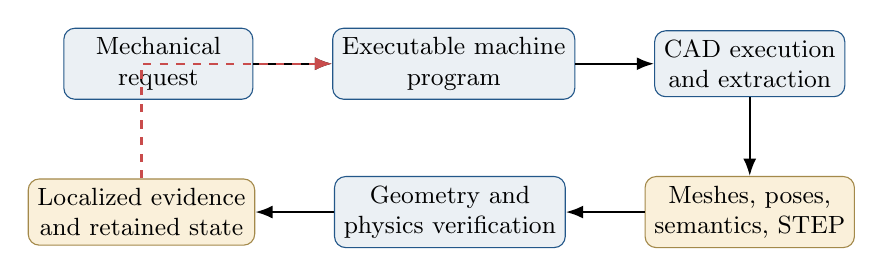
\begin{tikzpicture}[node distance=10mm and 10mm, font=\small]
  \node[process] (request) {Mechanical\\request};
  \node[process, right=of request] (program) {Executable machine\\program};
  \node[process, right=of program] (execute) {CAD execution\\and extraction};
  \node[state, below=of execute] (artifacts) {Meshes, poses,\\semantics, STEP};
  \node[process, left=of artifacts] (verify) {Geometry and\\physics verification};
  \node[state, left=of verify] (evidence) {Localized evidence\\and retained state};
  \draw[flow] (request) -- (program);
  \draw[flow] (program) -- (execute);
  \draw[flow] (execute) -- (artifacts);
  \draw[flow] (artifacts) -- (verify);
  \draw[flow] (verify) -- (evidence);
  \draw[feedback] (evidence) |- (program);
\end{tikzpicture}
\caption{AutoMech converts a request into executable program state, evaluates that state,
and closes the loop with measured evidence.}
\label{fig:architecture}
\end{figure}

\subsection{Parametric Program Representation}

\subsubsection{Executable geometric representation}

The generated response contains one Python block whose \CodeRef{build_machine()} function
constructs the complete assembly. The runtime injects the CAD library, selected modeling
primitives, \CodeRef{AssemblyHelper}, and a toothed gear constructor. The function must
return a compound with named leaves; only leaves with positive solid volume become realized
parts \CodeRef{maker2/_eval_runner_machine.py:7--15,47--62,83--128}.

The representation is deliberately parametric. Root parameters encode independent design
choices such as module, tooth counts, shaft radius, face width, wall thickness, and fit
clearance. Derived functions encode their consequences. A compact example is:

\begin{lstlisting}
module = 0.8
z_input, z_output = 12, 36
shaft_radius = 4.0
running_clearance = 0.05

def pitch_radius(z):
    return module * z / 2.0

def center_distance(z_a, z_b):
    return pitch_radius(z_a) + pitch_radius(z_b)

output_x = center_distance(z_input, z_output)
bearing_bore_radius = shaft_radius + running_clearance
\end{lstlisting}

For module $m$ and tooth count $z$, the pitch radius and external-mesh center distance are
\begin{equation}
  r_p(z)=\frac{mz}{2}, \qquad
  a_{12}=r_p(z_1)+r_p(z_2)=\frac{m(z_1+z_2)}{2}.
  \label{eq:gear-geometry}
\end{equation}
The ideal external-gear velocity relation is
\begin{equation}
  \frac{\omega_2}{\omega_1}=-\frac{z_1}{z_2}.
  \label{eq:gear-ratio}
\end{equation}

The significance of Equations~\ref{eq:gear-geometry}--\ref{eq:gear-ratio} is their location.
When the relationship exists only in hidden reasoning, a later coordinate can silently
disagree. When it exists in the generated Python, execution preserves the dependency and
review can inspect it. The same rule applies to axial stations, bores, hardpoints, housing
envelopes, and swept clearances \CodeRef{maker2/prompts/single_agent_prompt.py:24--41}.

\subsubsection{Mechanism semantic representation}

Shape alone does not determine mechanical intent. The same cylinder can be a fixed post, a
rotating arbor, or a sliding plunger. AutoMech therefore places a plain Python
\CodeRef{MECHANISM} dictionary beside the geometry function. Table~\ref{tab:semantics}
summarizes the implemented semantic groups.

\begin{table}[ht]
\centering
\caption{Semantic groups in the authored machine program.}
\label{tab:semantics}
\begin{tabularx}{\linewidth}{@{}lX@{}}
\toprule
Group & Purpose \\
\midrule
Ports & Named local attachment, bore, shaft, mesh, face, and cylindrical features. \\
Relations & Geometric or closure connections between named ports. \\
Motion joints & Parent-dependent hinge or slide frames for serial moving structures. \\
Transmissions & Speed coupling between driving and driven links. \\
Planetary stages & Sun, planet, ring, carrier, tooth-count, and role declarations. \\
Output and watch links & Intended functional endpoint and bodies observed during testing. \\
\bottomrule
\end{tabularx}
\end{table}

Structural support, inherited motion, closure constraints, and transmission coupling are
separate semantics. A support name identifies what physically carries a part. A motion
joint identifies the moving coordinate frame. A closure relation constrains mechanisms
with multiple endpoints. A transmission identifies how motion should propagate. The
semantic sidecar and generated assembly must reference the same realized names
\CodeRef{maker2/prompts/single_agent_prompt.py:69--172}.

\subsection{Execution and Normalization}

\subsubsection{Time-bounded program execution}

The authored block is written to \CodeRef{machine.py} and evaluated by a dedicated child
process with a five-minute timeout \CodeRef{maker2/single_agent.py:27--28,364--386}. The
runner executes the program, obtains the built compound, traverses its leaves, and
serializes either a valid payload or an exception. This boundary gives operational process
isolation and time bounding. It is not presented as a formally hardened security boundary.

Geometry-kernel failures can carry little actionable text. AutoMech therefore searches the
traceback for the final frame inside \CodeRef{machine.py} and reports its line, function,
and source expression. This maps an opaque native exception to the program location the
agent can actually edit \CodeRef{maker2/single_agent.py:35--50}.

\subsubsection{Local geometry and world pose}

Each built leaf has an assembled world location. Before STL export, the runner removes the
leaf's own placement, producing a mesh in the part-local frame. The assembled rotation
$\mathbf R_i$ and translation $\mathbf t_i$ are recorded separately
\CodeRef{maker2/_eval_runner_machine.py:101--125}. A local vertex is assembled by
\begin{equation}
  \mathbf v_W=\mathbf R_i\mathbf v_L+\mathbf t_i.
  \label{eq:world-transform}
\end{equation}
A parent-relative transform can be recovered from world transforms as
\begin{equation}
  \mathbf T_{P\rightarrow i}=\mathbf T_P^{-1}\mathbf T_i.
  \label{eq:relative-transform}
\end{equation}

This separation prevents a transform from being baked into a mesh and then applied again
by downstream consumers. The evaluation payload records part name, rotation, translation,
metadata, relative mesh path, volume, and local bounding box. Selected mechanism fields
are copied from the sidecar, and a whole-machine STEP file is exported for later precision
inspection \CodeRef{maker2/_eval_runner_machine.py:128--149}.

\begin{figure}[ht]
\centering
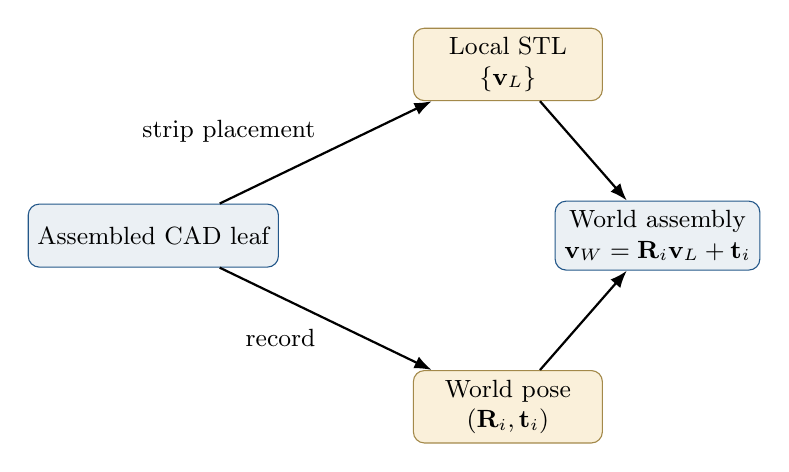
\begin{tikzpicture}[node distance=13mm and 17mm, font=\small]
  \node[process] (leaf) {Assembled CAD leaf};
  \node[state, above right=of leaf] (local) {Local STL\\$\{\mathbf v_L\}$};
  \node[state, below right=of leaf] (pose) {World pose\\$(\mathbf R_i,\mathbf t_i)$};
  \node[process, right=35mm of leaf] (world) {World assembly\\$\mathbf v_W=\mathbf R_i\mathbf v_L+\mathbf t_i$};
  \draw[flow] (leaf) -- node[above left]{strip placement} (local);
  \draw[flow] (leaf) -- node[below left]{record} (pose);
  \draw[flow] (local) -- (world);
  \draw[flow] (pose) -- (world);
\end{tikzpicture}
\caption{AutoMech stores shape in a local frame and assembly placement explicitly.}
\label{fig:frames}
\end{figure}

\subsection{Simulator-Facing Representation}

AutoMech normalizes evaluated parts and semantic declarations into a typed mechanism model.
This intermediate representation separates authoring syntax from simulation semantics. It
contains links, poses, ports, relations, motion joints, transmissions, planetary stages,
an intended output, and watch links. Robot and simulator descriptions are derived from this
state rather than inferred independently from prose.

The normalized representation provides three practical invariants. First, names remain
stable across meshes, relations, logs, and metrics. Second, local geometry and world pose
remain separate. Third, physical evaluation reads explicit function intent---for example,
which input is driven and which downstream bodies should move---instead of judging motion
from arbitrary visual change.

\subsection{Verification and Reward System}

AutoMech uses deterministic checks and measured physical behavior as a reward system for
revision. Here, ``reward'' means an external control signal used to order generated states;
it is not a learned scalar model and not a benchmark result.

\subsubsection{Assembly-consistency alignment}

Before expensive solid checks, AutoMech constructs an undirected proximity supergraph over
evaluated meshes. Two parts receive an edge when their world-space mesh distance is below
$\tau=10\,\mathrm{mm}$; overlapping axis-aligned boxes are admitted immediately. Let $V$
be realized parts, $E_\tau$ proximity edges, and $D$ the recognized declared support and
mesh edges. The gate accepts only if
\begin{equation}
  \operatorname{connected}(G_\tau) \quad\land\quad D\subseteq E_\tau,
  \qquad G_\tau=(V,E_\tau).
  \label{eq:connectivity}
\end{equation}

The graph is intentionally permissive. Passing is not a proof of correct assembly. Failing
is stronger evidence: even the over-connected graph is split, or a declaration names parts
that are not within a broad geometric tolerance
\CodeRef{maker2/single_agent.py:53--211}.

\subsubsection{Geometry regularization}

After connectivity, AutoMech checks gross rigid interpenetration on realized solids.
Intended adjacency and recognized fits receive targeted exemptions; unrelated solid volume
is not excused. Abstractly, a conflict remains when
\begin{equation}
  \operatorname{vol}(A_i\cap A_j)>\varepsilon
  \label{eq:intersection}
\end{equation}
after permitted-pair rules are applied \CodeRef{maker2/subcheck.py:240--303}.

A large machine can produce more pairwise findings than a feedback turn can use. The
implementation greedily groups conflicts around the part that participates in the most
remaining pairs. One diagnostic then reports that likely shared cause---wrong size, origin,
or placement---instead of asking the agent to move every affected neighbor
\CodeRef{maker2/single_agent.py:703--754}. A development incident documented in source
comments observed a list truncated to 8 of 63 pairs and a later state with 39 conflicts
across 41 parts. These are debugging observations, not evaluation results.

\subsubsection{Functional alignment}

Physical evaluation measures whether the machine performs its intended motion. Relevant
signals include input travel, moved and watched part counts, output reach, explosion state,
tilt, drift, bore-fit faults, and interferences. A stable object that transmits no motion
should not outrank a slightly imperfect mechanism that propagates drive.

Let $n_m$ be moved parts, $n_w$ watched parts, $I_o$ indicate output reach, and $q_{in}$ be
input travel. The current search-control score is
\begin{equation}
S_i=
\begin{cases}
10000, & \text{if the evaluated mechanism passes},\\
-100+100\min\!\left(1,\dfrac{n_m}{\max(1,n_w)}\right), & \text{if it explodes},\\
b+4000I_o+3000\rho_m+800\rho_{in}, & \text{otherwise},
\end{cases}
\label{eq:control-score}
\end{equation}
where
\begin{equation}
 b=\begin{cases}200,&\text{stable},\\-500,&\text{unstable},\end{cases}
 \quad
 \rho_m=\begin{cases}\min(1,n_m/n_w),&n_w>0,\\0,&n_w=0,\end{cases}
 \quad
 \rho_{in}=\min(1,q_{in}/10).
\end{equation}

This score controls candidate retention inside one run. It is not calibrated for comparing
unrelated benchmark tasks \CodeRef{maker2/single_agent.py:609--662}.

% -----------------------------------------------------------------------------
\section{AutoMech Framework}
% -----------------------------------------------------------------------------

The AutoMech framework turns the architecture above into a repeatable synthesis and
refinement procedure. Its three stages mirror the role played by infrastructure, initial
optimization, and feedback-driven optimization in large-system technical reports, but all
three stages operate on one authored whole-machine program.

\subsection{Framework Infrastructure}

A run creates an isolated artifact directory and a persistent \CodeRef{run.log}. The
conversation begins from a textual request and may include one reference image in the
first authoring turn. The image is not resent during revision because later turns operate
on evidence from the agent's own generated machine
\CodeRef{maker2/single_agent.py:798--862}.

The core infrastructure consists of:
\begin{itemize}[leftmargin=*]
  \item a conversation state carrying the authored program and subsequent evidence;
  \item a child-process CAD evaluator with a fixed execution timeout;
  \item a normalized artifact contract for local meshes, poses, semantics, and simulator
        descriptions;
  \item deterministic geometry checks and physical evaluation;
  \item per-iteration artifact snapshots and a separately retained best state; and
  \item structured progress and diagnosis events for the surrounding application.
\end{itemize}

The authoring loop has a configurable iteration cap. A nonpositive user cap selects an
implementation hard ceiling, preventing pathological unlimited execution. Each iteration
must produce an executable state before it can advance to geometric or physical checks
\CodeRef{maker2/single_agent.py:892--925}.

\subsection{Initial Machine Synthesis}

Initial synthesis asks the agent for short design notes followed by one Python block. The
program must define root parameters and derived calculations before constructing dependent
geometry. It then creates every real part, assigns a stable name and metadata, and returns
one complete assembly. Mechanism semantics are declared beside the geometry under the same
part names.

The synthesized program is evaluated immediately. Missing code blocks, absent required
functions, child-process exceptions, empty solids, and robot-description construction
failures are returned as build evidence. No later check treats unexecuted source as a valid
machine. Once execution succeeds, AutoMech freezes the iteration before working filenames
can be overwritten \CodeRef{maker2/single_agent.py:923--975}.

Figure~\ref{fig:executable-reasoning} highlights the main distinction from free-form
reasoning: root choices flow through executable derivations into both geometry and
semantics.

\begin{figure}[ht]
\centering
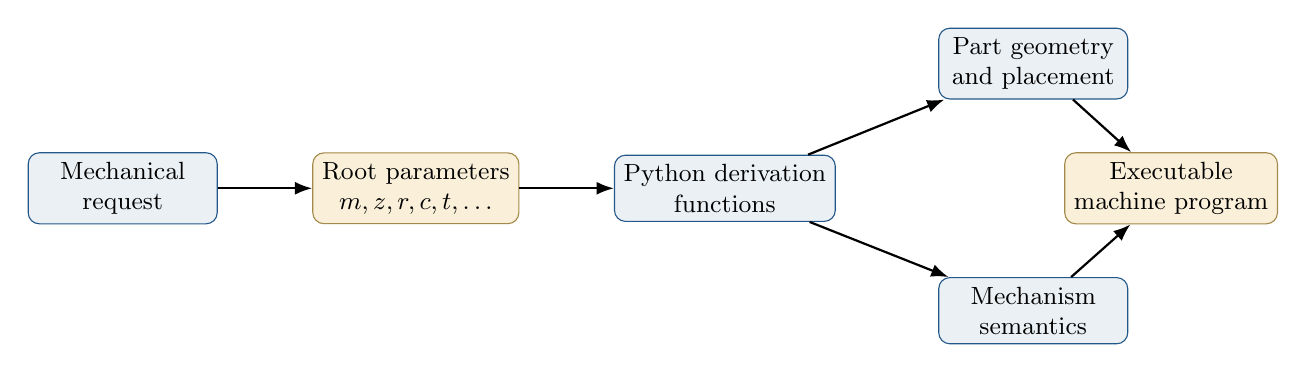
\begin{tikzpicture}[node distance=11mm and 12mm, font=\small]
  \node[process] (req) {Mechanical\\request};
  \node[state, right=of req] (root) {Root parameters\\$m,z,r,c,t,\ldots$};
  \node[process, right=of root] (derive) {Python derivation\\functions};
  \node[process, above right=7mm and 13mm of derive] (geom) {Part geometry\\and placement};
  \node[process, below right=7mm and 13mm of derive] (sem) {Mechanism\\semantics};
  \node[state, right=29mm of derive] (machine) {Executable\\machine program};
  \draw[flow] (req) -- (root);
  \draw[flow] (root) -- (derive);
  \draw[flow] (derive) -- (geom);
  \draw[flow] (derive) -- (sem);
  \draw[flow] (geom) -- (machine);
  \draw[flow] (sem) -- (machine);
\end{tikzpicture}
\caption{Mechanical dependencies are materialized as executable expressions before they
feed geometry and semantic metadata.}
\label{fig:executable-reasoning}
\end{figure}

\subsection{Verification-Guided Refinement}

Refinement proceeds through the sequence in Figure~\ref{fig:framework-loop}. Build errors
return first because no geometric state exists. A successful build enters connectivity and
intersection checks. A geometrically admissible state enters physical evaluation. Only a
verified machine-domain failure becomes a CAD revision request; an evaluation-system fault
halts instead of causing an unrelated rewrite \CodeRef{maker2/single_agent.py:1035--1074}.

\begin{figure}[p]
\centering
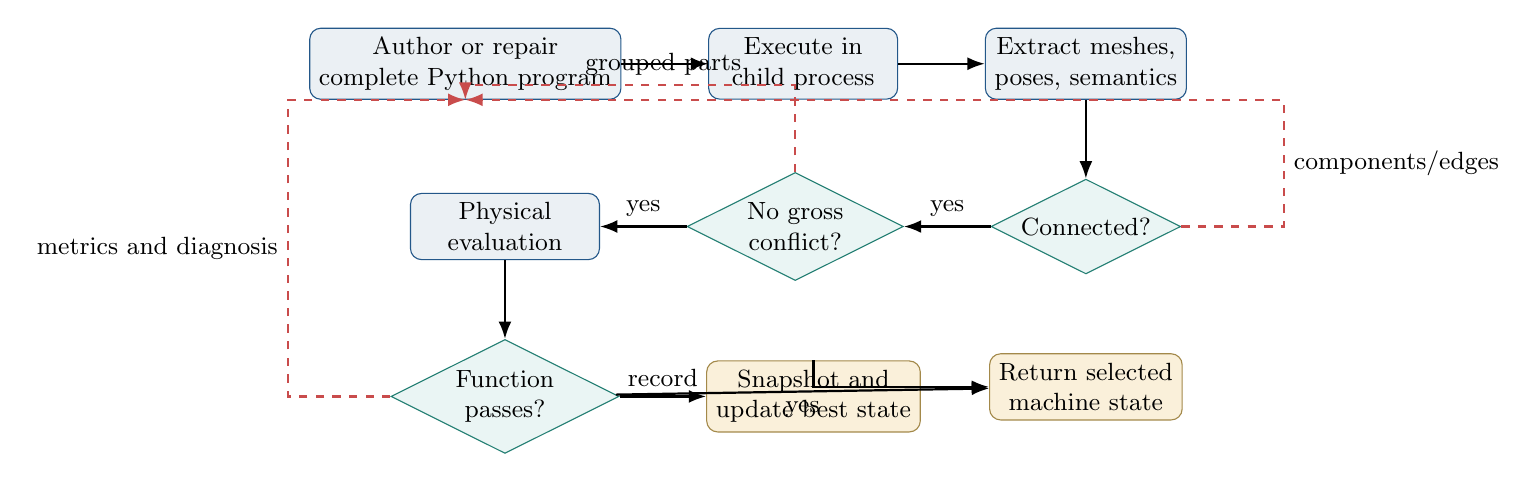
\begin{tikzpicture}[node distance=10mm and 11mm, font=\small]
  \node[process] (author) {Author or repair\\complete Python program};
  \node[process, right=of author] (exec) {Execute in\\child process};
  \node[process, right=of exec] (extract) {Extract meshes,\\poses, semantics};
  \node[check, below=of extract] (conn) {Connected?};
  \node[check, left=of conn] (overlap) {No gross\\conflict?};
  \node[process, left=of overlap] (phys) {Physical\\evaluation};
  \node[check, below=of phys] (pass) {Function\\passes?};
  \node[state, right=of pass] (snap) {Snapshot and\\update best state};
  \node[state, below=of conn] (done) {Return selected\\machine state};

  \draw[flow] (author) -- (exec);
  \draw[flow] (exec) -- (extract);
  \draw[flow] (extract) -- (conn);
  \draw[flow] (conn) -- node[above]{yes} (overlap);
  \draw[flow] (overlap) -- node[above]{yes} (phys);
  \draw[flow] (phys) -- (pass);
  \draw[flow] (pass) -- node[above]{record} (snap);
  \draw[flow] (snap) |- (done);
  \draw[feedback] (conn.east) -- ++(13mm,0) |- node[pos=0.25,right]{components/edges} (author.south);
  \draw[feedback] (overlap.north) -- ++(0,11mm) -| node[pos=0.2,above]{grouped parts} (author.south);
  \draw[feedback] (pass.west) -- ++(-13mm,0) |- node[pos=0.25,left]{metrics and diagnosis} (author.south);
  \draw[flow] (pass) -- node[below]{yes} (done);
\end{tikzpicture}
\caption{Verification-guided synthesis and revision in AutoMech.}
\label{fig:framework-loop}
\end{figure}

The revision instruction is deliberately local. It names observed faulty parts, asks for
the smallest parameter edit, preserves identifiers, and discourages restructuring. If a
new geometry has more rigid conflicts than the best prior geometry, the next turn receives
the best geometry code rather than the worse recent code
\CodeRef{maker2/prompts/single_agent_prompt.py:296--332}.

Physical refinement tracks which impossible fits were fixed and which were introduced by
the newest edit. This delta prevents the next instruction from undoing successful changes
merely because the overall mechanism still fails \CodeRef{maker2/single_agent.py:1115--1144}.

Two retained objectives control divergence:
\begin{itemize}[leftmargin=*]
  \item \textbf{geometry best}: the state with the fewest rigid conflicts; and
  \item \textbf{physics best}: the state with the highest functional control score.
\end{itemize}
The selected physical state is
\begin{equation}
  i^\star=\arg\max_i S_i.
  \label{eq:best-state}
\end{equation}
Each completed build is copied under \CodeRef{iter_<n>/}. A separate best directory retains
the highest-scoring script and normalized descriptions
\CodeRef{maker2/single_agent.py:665--700,1076--1155}. The visible restore path copies the
script, typed model, and robot description, with a fallback that rebuilds from retained
code. Exact mesh-level atomic restoration requires explicit verification before it can be
claimed \CodeRef{maker2/single_agent.py:757--787}.

\begin{figure}[ht]
\centering
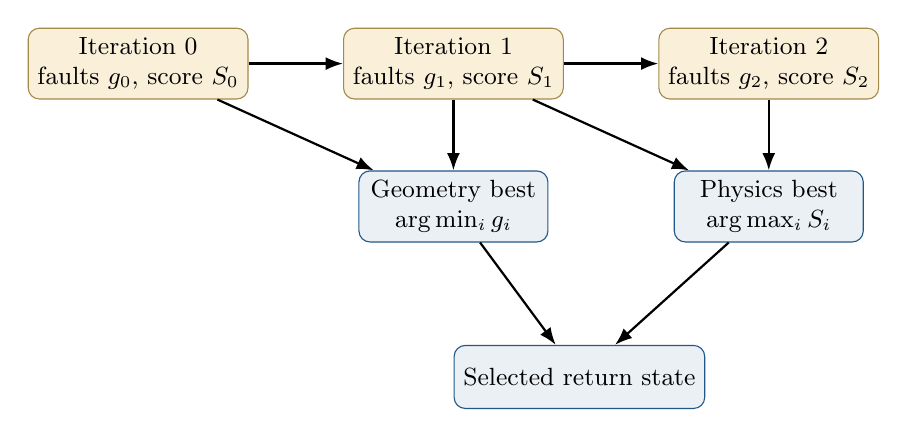
\begin{tikzpicture}[node distance=9mm and 12mm, font=\small]
  \node[state] (i0) {Iteration 0\\faults $g_0$, score $S_0$};
  \node[state, right=of i0] (i1) {Iteration 1\\faults $g_1$, score $S_1$};
  \node[state, right=of i1] (i2) {Iteration 2\\faults $g_2$, score $S_2$};
  \node[process, below=of i1] (gb) {Geometry best\\$\arg\min_i g_i$};
  \node[process, below=of i2] (pb) {Physics best\\$\arg\max_i S_i$};
  \node[process, below=13mm of gb, xshift=16mm] (sel) {Selected return state};
  \draw[flow] (i0) -- (i1);
  \draw[flow] (i1) -- (i2);
  \draw[flow] (i0) -- (gb);
  \draw[flow] (i1) -- (gb);
  \draw[flow] (i1) -- (pb);
  \draw[flow] (i2) -- (pb);
  \draw[flow] (gb) -- (sel);
  \draw[flow] (pb) -- (sel);
\end{tikzpicture}
\caption{Per-iteration persistence and two levels of best-state retention.}
\label{fig:retention}
\end{figure}

% -----------------------------------------------------------------------------
\section{Evaluation}
% -----------------------------------------------------------------------------

\PendingResultsNotice

Evaluation should separate buildability, geometric consistency, physical evaluability,
and functional success. A run that emits geometry but cannot be simulated is not equivalent
to a functional pass. The internal control score in Equation~\ref{eq:control-score} must not
be reported as a cross-task quality score.

\subsection{Evaluation Metrics}

Table~\ref{tab:metrics} defines the proposed metric families. Outcome values are populated
only from retained artifacts after controlled execution.

\begin{table}[ht]
\centering
\caption{Evaluation metric families.}
\label{tab:metrics}
\begin{tabularx}{\linewidth}{@{}lX@{}}
\toprule
Family & Definition \\
\midrule
Execution & Presence of an executable script and nonempty realized part set. \\
Assembly consistency & Connectivity of $G_\tau$ and realization of declared edges $D$. \\
Geometry & Absence or count of nonexempt rigid solid intersections. \\
Physical evaluability & Simulator model loads and emits a complete metrics contract. \\
Function & Input travels, downstream links move, and intended output is reached. \\
Refinement & Iterations, regression events, rollback use, and final selected state. \\
Efficiency & Wall-clock time and retained artifact volume under fixed conditions. \\
\bottomrule
\end{tabularx}
\end{table}

Aggregate rates may be defined as
\begin{align}
 R_{\mathrm{build}} &= \frac{N_{\mathrm{buildable}}}{N_{\mathrm{attempted}}},\\
 R_{\mathrm{physics}} &= \frac{N_{\mathrm{physics\ pass}}}{N_{\mathrm{physics\ evaluable}}},\\
 R_{\mathrm{rollback}} &= \frac{N_{\mathrm{runs\ with\ rollback}}}{N_{\mathrm{completed\ runs}}}.
\end{align}
If a denominator is zero, the corresponding result remains blank rather than being
reported as zero.

\subsection{Scaling}

\subsubsection{Part-count scaling}

The primary scaling axis is realized part count, with explicit attention to the $21+$ band.
The protocol should hold task-set revision, iteration policy, CAD configuration, physical
evaluation configuration, and hardware conditions fixed.

\PendingResultsNotice
\begin{table}[ht]
\centering
\caption{Scaling template. All outcome columns are intentionally blank.}
\small
\begin{tabularx}{\linewidth}{@{}l*{6}{>{\centering\arraybackslash}X}@{}}
\toprule
Parts & Build completion & Connectivity & Conflict-free & Physics-ready & Functional pass & Runtime \\
\midrule
1--5   & \ResultBlank & \ResultBlank & \ResultBlank & \ResultBlank & \ResultBlank & \ResultBlank \\
6--10  & \ResultBlank & \ResultBlank & \ResultBlank & \ResultBlank & \ResultBlank & \ResultBlank \\
11--20 & \ResultBlank & \ResultBlank & \ResultBlank & \ResultBlank & \ResultBlank & \ResultBlank \\
21+    & \ResultBlank & \ResultBlank & \ResultBlank & \ResultBlank & \ResultBlank & \ResultBlank \\
\bottomrule
\end{tabularx}
\end{table}

\subsubsection{Executable input representation}

This study isolates whether explicit root parameters and derived functions reduce drift
relative to independently written dependent literals. The evaluated program must remain
otherwise comparable, and all outcome fields remain blank until execution.

\PendingResultsNotice
\begin{table}[ht]
\centering
\caption{Executable-representation study template.}
\small
\begin{tabularx}{\linewidth}{@{}X*{4}{>{\centering\arraybackslash}X}@{}}
\toprule
Representation & Build completion & Geometry pass & Functional pass & Iterations \\
\midrule
Root parameters with derivations & \ResultBlank & \ResultBlank & \ResultBlank & \ResultBlank \\
Independent dependent literals & \ResultBlank & \ResultBlank & \ResultBlank & \ResultBlank \\
\bottomrule
\end{tabularx}
\end{table}

\subsection{Verification-Guided Refinement}

\subsubsection{Assembly-consistency alignment}

This ablation measures the effect of checking the permissive proximity graph and declared
edges before solid-intersection analysis.

\PendingResultsNotice
\begin{table}[ht]
\centering
\caption{Assembly-consistency ablation template.}
\small
\begin{tabularx}{\linewidth}{@{}X*{4}{>{\centering\arraybackslash}X}@{}}
\toprule
Configuration & Disconnected builds & Geometry pass & Functional pass & Iterations \\
\midrule
Connectivity check enabled & \ResultBlank & \ResultBlank & \ResultBlank & \ResultBlank \\
Connectivity check disabled & \ResultBlank & \ResultBlank & \ResultBlank & \ResultBlank \\
\bottomrule
\end{tabularx}
\end{table}

\subsubsection{Geometry regularization}

This study compares cause-grouped intersection feedback with an ungrouped pair list while
preserving the same underlying solid-intersection detector.

\PendingResultsNotice
\begin{table}[ht]
\centering
\caption{Geometry-feedback ablation template.}
\small
\begin{tabularx}{\linewidth}{@{}X*{4}{>{\centering\arraybackslash}X}@{}}
\toprule
Feedback & Conflict-free & Fault reduction & Regressions & Iterations \\
\midrule
Cause-grouped feedback & \ResultBlank & \ResultBlank & \ResultBlank & \ResultBlank \\
Ungrouped pair feedback & \ResultBlank & \ResultBlank & \ResultBlank & \ResultBlank \\
\bottomrule
\end{tabularx}
\end{table}

\subsubsection{Functional alignment}

This study isolates physical feedback and function-dominated retention. It must distinguish
a physically unevaluable run from a mechanism that evaluates and fails.

\PendingResultsNotice
\begin{table}[ht]
\centering
\caption{Functional-alignment ablation template.}
\small
\begin{tabularx}{\linewidth}{@{}X*{4}{>{\centering\arraybackslash}X}@{}}
\toprule
Configuration & Physics-ready & Output reached & Rollback & Iterations \\
\midrule
Physical feedback and best retention & \ResultBlank & \ResultBlank & \ResultBlank & \ResultBlank \\
Geometry-only refinement & \ResultBlank & \ResultBlank & \ResultBlank & \ResultBlank \\
\bottomrule
\end{tabularx}
\end{table}

\subsection{Artifact Integrity}

A report-level evaluation should verify that each visible iteration refers to its own
script, normalized state, robot description, and meshes rather than aliases of the final
working filenames. It should separately test whether restoring the retained best state
reconstructs an artifact set with matching hashes and loadable references.

\PendingResultsNotice
\begin{table}[ht]
\centering
\caption{Artifact-integrity template.}
\small
\begin{tabularx}{\linewidth}{@{}l*{5}{>{\centering\arraybackslash}X}@{}}
\toprule
Task & Unique iterations & Mesh match & Model loads & Best restores & Log complete \\
\midrule
\ResultBlank & \ResultBlank & \ResultBlank & \ResultBlank & \ResultBlank & \ResultBlank \\
\ResultBlank & \ResultBlank & \ResultBlank & \ResultBlank & \ResultBlank & \ResultBlank \\
\bottomrule
\end{tabularx}
\end{table}

\subsection{Controlled Benchmark Protocol}

Before any result is added, the run metadata in Table~\ref{tab:run-metadata} must be frozen.
Future values may be populated only from retained run directories and checked aggregation
scripts, never from source-code control flow or development anecdotes.

\PendingResultsNotice
\begin{table}[ht]
\centering
\caption{Run metadata template.}
\label{tab:run-metadata}
\begin{tabularx}{\linewidth}{@{}lXlX@{}}
\toprule
Field & Value & Field & Value \\
\midrule
Execution date & \ResultBlank & Commit & \ResultBlank \\
Local-change state & \ResultBlank & Task-set revision & \ResultBlank \\
Part-count band & \ResultBlank & CAD configuration & \ResultBlank \\
Physics configuration & \ResultBlank & Iteration cap & \ResultBlank \\
Repetitions & \ResultBlank & Hardware summary & \ResultBlank \\
\bottomrule
\end{tabularx}
\end{table}

\PendingResultsNotice
\begin{table}[ht]
\centering
\caption{Per-task result template.}
\small
\begin{tabularx}{\linewidth}{@{}l*{7}{>{\centering\arraybackslash}X}@{}}
\toprule
Task & Parts & Script & Connected & Conflict-free & Physics-ready & Output reached & Iterations \\
\midrule
\ResultBlank & \ResultBlank & \ResultBlank & \ResultBlank & \ResultBlank & \ResultBlank & \ResultBlank & \ResultBlank \\
\ResultBlank & \ResultBlank & \ResultBlank & \ResultBlank & \ResultBlank & \ResultBlank & \ResultBlank & \ResultBlank \\
\ResultBlank & \ResultBlank & \ResultBlank & \ResultBlank & \ResultBlank & \ResultBlank & \ResultBlank & \ResultBlank \\
\bottomrule
\end{tabularx}
\end{table}

% -----------------------------------------------------------------------------
\section{Conclusion, Limitations, and Future Directions}
% -----------------------------------------------------------------------------

AutoMech preserves the directness of whole-machine text-to-CAD while changing where
mechanical reasoning lives. Dimensions and placements that determine correctness are
encoded as executable dependencies over root parameters. The authored program is executed,
not merely read; local geometry and world pose are separated; semantic intent is retained
in structured form; deterministic checks and physical measurements produce localized
feedback; and snapshots prevent a recent regression from erasing a better state.

The current implementation has important limitations:
\begin{enumerate}[leftmargin=*]
  \item \textbf{Complete-source replacement.} Feedback is localized, but the generation
        interface still returns a complete replacement program rather than a source patch.
  \item \textbf{Execution boundary.} Child-process isolation and timeout improve operational
        control but do not constitute a proof of security against malicious native code.
  \item \textbf{Conservative connectivity.} The proximity graph intentionally admits false
        edges and verifies only currently recognized support and mesh declarations.
  \item \textbf{Distinct control signals.} Intersection count and functional score have
        different meanings and must not be combined as if they shared a scale.
  \item \textbf{Best-effort evaluation.} Some paths may retain a geometrically built artifact
        when physical evaluation itself errors; this is not a physical pass.
  \item \textbf{Restoration atomicity.} Exact restoration of every mesh belonging to the
        retained best state requires explicit verification before it can be claimed.
  \item \textbf{Development evidence.} Historical incidents explain design choices but do
        not estimate general performance.
\end{enumerate}

Future work should evaluate the blank protocol, especially the $21+$ part-count band;
replace complete-source transport with constrained patches where practical; broaden
semantic consistency checks beyond the currently recognized edges; verify atomic best-state
restoration; and calibrate control objectives on labeled mechanical outcomes. No claim of
higher success, quality, speed, or reliability is made before those measurements exist.

\appendix

% -----------------------------------------------------------------------------
\section{Implementation Details}
% -----------------------------------------------------------------------------

\begin{longtable}{@{}p{0.27\linewidth}p{0.65\linewidth}@{}}
\caption{Principal AutoMech artifacts.}\label{tab:artifacts}\\
\toprule
Artifact & Role \\
\midrule
\endfirsthead
\toprule
Artifact & Role \\
\midrule
\endhead
\CodeRef{machine.py} & Complete authored geometry and mechanism program. \\
\CodeRef{_machine_runner.py} & Per-run copy of the child-process execution harness. \\
\CodeRef{machine_eval.json} & Evaluated parts, local mesh references, world transforms, and selected semantics. \\
\CodeRef{machine.step} & Whole-machine CAD exchange artifact for precision inspection. \\
\CodeRef{meshes/*.stl} & Per-part local-frame geometry. \\
\CodeRef{kinematic_model.json} & Typed normalized mechanism representation. \\
\CodeRef{model.urdf} and simulator model & Robot and physical representations derived from normalized state. \\
\CodeRef{iter_<n>/} & Frozen geometry and description for one completed build attempt. \\
\CodeRef{best/} & Retained highest-scoring script and normalized state. \\
\CodeRef{run.log} & Persistent authoring, checking, simulation, and diagnosis trace. \\
Physical artifacts & Metrics, diagnosis, contact preparation, frames, and optional video. \\
Run/result metadata & Final status and paths consumed by the surrounding application. \\
\bottomrule
\end{longtable}

\begin{longtable}{@{}p{0.34\linewidth}p{0.58\linewidth}@{}}
\caption{Implementation evidence index.}\label{tab:evidence}\\
\toprule
Claim & Repository evidence \\
\midrule
\endfirsthead
\toprule
Claim & Repository evidence \\
\midrule
\endhead
Whole-machine program contract & \CodeRef{maker2/prompts/single_agent_prompt.py:1--17,43--67} \\
Executable root and derived arithmetic & \CodeRef{maker2/prompts/single_agent_prompt.py:24--41} \\
Structured mechanism semantics & \CodeRef{maker2/prompts/single_agent_prompt.py:69--172} \\
Program evaluation loop & \CodeRef{maker2/single_agent.py:798--959} \\
Child-process runner & \CodeRef{maker2/_eval_runner_machine.py:1--62} \\
Local mesh and world pose extraction & \CodeRef{maker2/_eval_runner_machine.py:73--128} \\
Whole-machine STEP export & \CodeRef{maker2/_eval_runner_machine.py:138--149} \\
Conservative connectivity & \CodeRef{maker2/single_agent.py:53--211,977--997} \\
Rigid-intersection check & \CodeRef{maker2/single_agent.py:999--1033}; \CodeRef{maker2/subcheck.py:240--303} \\
Cause-grouped feedback & \CodeRef{maker2/single_agent.py:703--754} \\
Minimal repair and geometry rollback & \CodeRef{maker2/prompts/single_agent_prompt.py:296--332} \\
Iteration snapshots & \CodeRef{maker2/single_agent.py:665--700,969--975} \\
Functional control score & \CodeRef{maker2/single_agent.py:609--662} \\
Physical feedback and routing & \CodeRef{maker2/single_agent.py:1035--1145} \\
Best-state restoration & \CodeRef{maker2/single_agent.py:757--787,1076--1155} \\
Large part-count collision preparation & \CodeRef{maker2/convex_decomp.py:357--373} \\
\bottomrule
\end{longtable}

% -----------------------------------------------------------------------------
\section{Benchmark Execution Details}
% -----------------------------------------------------------------------------

Before populating Section~4:
\begin{enumerate}[leftmargin=*]
  \item freeze the task set and its revision;
  \item record the exact implementation commit and local-change state;
  \item define fixed iteration and physical-evaluation policies;
  \item retain every run directory, log, snapshot, metric file, and diagnosis;
  \item distinguish execution, geometry, evaluation, and functional failures;
  \item compute aggregate values from artifacts with a checked script;
  \item preserve blank cells whenever a denominator or measurement is undefined; and
  \item remove pending-result notices only after every populated cell is traceable to
        retained evidence.
\end{enumerate}

% -----------------------------------------------------------------------------
\section{Case Study for Executable Reasoning}
% -----------------------------------------------------------------------------

\subsection{Representation Cases}

A dependent quantity should be represented as a function when changing one design decision
must update another value. Examples include:
\begin{itemize}[leftmargin=*]
  \item gear center distance as a function of module and tooth counts;
  \item bearing bore as shaft radius plus running clearance;
  \item a press-fit bore as shaft radius minus intended interference;
  \item an axial station as the previous station plus half-thicknesses and clearance;
  \item a shell inner envelope as the union of internal motion envelopes plus clearance; and
  \item a local port as the inverse part transform applied to a solved world hardpoint.
\end{itemize}

By contrast, aesthetic dimensions that are not mechanically coupled may remain independent
root parameters. The criterion is dependency, not whether a number appears simple.

\subsection{Revision Cases}

When one central part intersects many neighbors, pairwise repair suggests many edits. The
cause-grouped representation instead asks whether the central part has an incorrect origin,
size, or pose. When a new revision regresses, the retained-state representation changes the
next starting point from ``latest'' to ``best observed.'' When a physical failure includes
fit deltas, the next instruction preserves fits that were repaired and focuses on newly
broken or unchanged ones. These cases illustrate how representation determines whether a
revision loop accumulates progress or repeatedly re-rolls correct work.

% -----------------------------------------------------------------------------
\section{Notations}
% -----------------------------------------------------------------------------

\begin{table}[ht]
\centering
\caption{Notation used in this report.}
\begin{tabularx}{\linewidth}{@{}lX@{}}
\toprule
Symbol & Meaning \\
\midrule
$m$ & Gear module. \\
$z$ & Gear tooth count. \\
$r_p(z)$ & Pitch radius of a gear with tooth count $z$. \\
$a_{12}$ & Center distance between a meshing gear pair. \\
$\mathbf v_L,\mathbf v_W$ & A vertex in local and world coordinates. \\
$\mathbf R_i,\mathbf t_i$ & World rotation and translation of part $i$. \\
$G_\tau=(V,E_\tau)$ & Conservative part-proximity graph at tolerance $\tau$. \\
$D$ & Recognized declared support and mesh edges. \\
$A_i$ & Solid occupied by realized part $i$. \\
$S_i$ & Within-run functional control score for iteration $i$. \\
$g_i$ & Geometry fault count for iteration $i$. \\
$n_m,n_w$ & Moved and watched part counts. \\
$I_o$ & Indicator that the intended output was reached. \\
$q_{in}$ & Measured input travel. \\
\bottomrule
\end{tabularx}
\end{table}

\begin{thebibliography}{9}
\bibitem{onerec}
G. Zhou et al., ``OneRec Technical Report,'' arXiv:2506.13695, 2025.
The report is cited only as an organizational reference for the architecture--framework--
evaluation presentation used here.

\bibitem{automech-code}
AutoMech implementation snapshot, repository-local source files listed in
Table~\ref{tab:evidence}, inspected August 10, 2026.
\end{thebibliography}

\end{document}
